\newcommand{\zNormalizationPerformed}[1]
{
  \textcolor{red}{\\It is important to NOTE that RAVEN uses a Z-score normalization of the training data before
  constructing the \textit{#1} ROM:
\begin{equation}
  \mathit{\mathbf{X'}} = \frac{(\mathit{\mathbf{X}}-\mu )}{\sigma }
\end{equation}
 }
}

\subsection{Build RAVEN Input: \xmlNode{RomTrainer}}
\label{sub:ravenROM}
The \textbf{RomTrainer} step type performs the training of a Reduced Order Model (ROM), and the specifications of
this step must be defined within a \xmlNode{RomTrainer} block. ROMs, also known as a surrogate model,  are used
to lower the computational cost, reducing the number of needed points and prioritizing the area of the input space
that needs to be explored when the simulations using the high-fidelity codes are very expensive. ROMs can be
considered as an artificial representation of the link between the input and output spaces for a particular system.

In most of the cases of interest, the information that is sought is related to defining the failure boundaries of
a system with respect to perturbations in the input space. For this reason, in the development of RAVEN, it has been
given priority to the introduction of a class of supervised learning algorithms, which are usually referred to as
classifiers. A classifier is a reduced order model that is capable of representing the system behavior through a
binary response (failure/success). Currently, RAVEN supports around 40 different ROM methodologies. All these
supervised learning algorithms have been imported via an API from the Scikit-Learn library. In addition, the N-Dimensional
spline and the inverse weight methods that are currently available for the interpolation of N-Dimensional PDF/CDF,
can also be used as ROMs.

In this section, the N-dimensional inverse weight method is employed to construct ROM to familarize the user with
the use of ROMs. Inverse distance weighting (IDW) is a type of deterministic method for multivariate interpolation
with a known scattered set of points. The assigned values to unknown points are calculated via a weighted average
of the values available at the known points.
\zNormalizationPerformed{NDinvDistWeight}
%%%%%%%%%%%%%%%%%%%%%%%%%%%%%%%%%%%%%%%%%%%%%%%%%%%%%%%%%%%%%%%%%%%%%
% Train and dump the rom
%%%%%%%%%%%%%%%%%%%%%%%%%%%%%%%%%%%%%%%%%%%%%%%%%%%%%%%%%%%%%%%%%%%%%
\subsubsection{How to train and output a ROM?}
In general, the ``training'' is a process that use sampling of the physical model to improve the prediction
capability of the ROM. As mentioned before, RAVEN provides lots of different sampling strategies, such as Monte
Carlo, Grid, Stratified (e.g. LHS), and Stochastic Collocation methods. All of them can be used to train a ROM.
In this section, we will continue to use \textbf{AnalyticBateman} to illustrate the setup of \textbf{RomTrainer}.
As before, a simple step \textbf{MultiRun} with \textbf{Monte Carlo} sampler is employed to generate the data set
that can be used to train the ROM. The full RAVEN input file can be found:
\textit{raven/tests/framework/user\_guide/ravenTutorial/RomTrain.xml}.
Because the setup of \textbf{MultiRun} is the same as previous example in section~\ref{sub:tutorialMultiRun}, the
RAVEN input file about the \textbf{MultiRun} is not include in this section. However, the full precedures are
listed here to make the user better understand the construction of ROM. The following precedures or RAVEN entities
are needed:

\begin{itemize}
  \item \textbf{MultiRun}: Monte Carlo sampling to generate the data set
  \begin{enumerate}
    \item Set up the running environment: \xmlNode{RunInfo};
    \item Provide the required files: \xmlNode{Files};
    \item Link between RAVEN and dirven code: \xmlNode{Code};
    \item Define probability distribution functions for inputs: \xmlNode{Distributions};
    \item Set up a simple Monte-Carlo sampling for perturbing the input space: \xmlNode{Samplers};
    \item Store the input and output data: \xmlNode{DataObjects};
    \item Print and plot input and output data: \xmlNode{OutStreams};
    \item Control multiple executions: \xmlNode{MultiRun}.
  \end{enumerate}
  \item \textbf{RomTrainer}: Train the ROM with given data set
  \begin{enumerate}
    \item Specify the type of ROMs: \xmlNode{ROM};
    \item Provide the data set for ROM training: \xmlNode{DataObjects};
    \item Train the ROM: \xmlNode{RomTrainer};
    \item Dump the ROM: \xmlNode{IOStep}
  \end{enumerate}
\end{itemize}

The specifications of the reduced order model must be defined within \xmlNode{ROM} XML block. This XML node accepts
the following attributes:

\begin{itemize}
  \itemsep0em
  \item \xmlAttr{name}, \xmlDesc{required string attribute}, user-defined identifier of this model.
  \item \xmlAttr{subType}, \xmlDesc{required string attribute}, defines which of
  the sub-types should be used, choosing among the previously reported types.
\end{itemize}
\vspace{-5mm}

In the \xmlNode{ROM} input block, the following XML sub-nodes are required,
independent of the \xmlAttr{subType} specified:
%
\begin{itemize}
   \item \xmlNode{Features}, \xmlDesc{comma separated string, required field}, specifies the names of the features
     of this ROM. \nb These parameters are going to be requested for the training of this object;
    \item \xmlNode{Target}, \xmlDesc{comma separated string, required field}, contains a comma separated list of
      the targets of this ROM. These parameters are the Figures of Merit (FOMs) this ROM is supposed to predict.
      \nb These parameters are going to be requested for the training of this object.
\end{itemize}

For each sub-type specified in the attribute \xmlAttr{subType}, additional sub-nodes may be required (Please check
the RAVEN user manual for each ROM). In addition, if an \xmlNode{HistorySet} is provided in the training step, then
a temporal ROM is created, i.e. a ROM that generates not a single value prediction of each element indicated in
the \xmlNode{Target} block but its full temporal profile. In this section, a time-dependent ROM will be constructed.

In order to use \textbf{N-dimensional inverse distance weighting} ROM, the \xmlNode{ROM} attribute \xmlAttr{subType}
needs to be \xmlString{NDinvDistWeight}. The following addition sub-node is also required.

\begin{itemize}
  \item \xmlNode{p}, \xmlDesc{integer, required field}, must be greater than zero and represents the
    ``power parameter''. For the choice of value for \xmlNode{p},it is necessary to consider the degree
    of smoothing desired in the interpolation/extrapolation, the density and distribution of samples being
    interpolated, and the maximum distance over which an individual sample is allowed to influence the
    surrounding ones (lower $p$ means greater importance for points far away).
\end{itemize}

Based on previous RAVEN input file used in section~\ref{sub:tutorialMultiRun}, the \xmlNode{ROM}, \xmlNode{RomTrain}
and \xmlNode{IOStep} are added. The \xmlNode{ROM} is used to describe the N-dimensional inverse distance weighting
ROM:
\xmlExample{framework/user_guide/ravenTutorial/RomTrain.xml}{Models}
The inputs and outputs of \textbf{AnalyticBateman} is used to generate the data set. The ROM will be constructed considering
two features (\textit{sigma-A and decay-A}) and two targets (\textit{A and time}). \nb the \textit{time} is treated
as target in ROM construction.

Then, the \xmlNode{RomTrain} and \xmlNode{IOStep} are used to construct ROM on the fly or dump the ROM into a file
(i.e. pickled ROM), respectively.
\xmlExample{framework/user_guide/ravenTutorial/RomTrain.xml}{Steps}
The \xmlString{HistorySet} generated by the \textbf{``sample''} step is used as input of the \textbf{``trainROM''}
step. The output of the \textbf{``trainROM''} is ``rom'' which is predefined in \xmlNode{ROM}. If a \xmlString{PointSet}
is provided as input, the output ``rom'' will be time-independent. The \textbf{``dumpROM''} step is used to serialize
the ``rom'' to file (pickled). In this example, the file is identified in \xmlNode{Files}.
\xmlExample{framework/user_guide/ravenTutorial/RomTrain.xml}{Files}
A pickled file with name ``inverseRom.pk'' will be generated in the working directory. This pickled ROM can be
reused by RAVEN to perform additional analysis, and we will introduce this capability in the following section.
Since we have four different steps to execute, the \xmlNode{RunInfo} block is modified:
\xmlExample{framework/user_guide/ravenTutorial/RomTrain.xml}{RunInfo}
The \xmlNode{Sequence} is used to provide an ordered list of the step names that RAVEN will run.

%%%%%%%%%%%%%%%%%%%%%%%%%%%%%%%%%%%%%%%%%%%%%%%%%%%%%%%%%%%%%%%%%%%%%
% Dump and sample the rom
%%%%%%%%%%%%%%%%%%%%%%%%%%%%%%%%%%%%%%%%%%%%%%%%%%%%%%%%%%%%%%%%%%%%%
\subsubsection{How to load and sample a ROM?}
In previous section, we have shown that RAVEN can be used to train a ROM and output the ROM to a pickled file. In
this section, we will show the user how to load the pickled ROM, and how to reuse it inside RAVEN environment.
In general, a \xmlNode{ROM} with subtype \xmlString{pickledROM} is used to hold the place of the ROM that will be
loaded from file. The notation for this ROM is much less than a typical ROM; it only requires a name and its subtype.

\textbf{Example:}
For this example the ROM has already been created and trained in another RAVEN run, then pickled to a file
called \texttt{rom\_pickle.pk}.  In the example, the file is identified in \xmlNode{Files}, the model is
defined in \xmlNode{Models}, and the model loaded in \xmlNode{Steps}.
{\footnotesize
\begin{lstlisting}[style=XML,morekeywords={name,subType}]
<Simulation>
  ...
  <Files>
    <Input name="rompk" type="">rom_pickle.pk</Input>
  </Files>
  ...
  <Models>
    ...
    <ROM name="myRom" subType="pickledROM"/>
    ...
  </Models>
  ...
  <Steps>
    ...
    <IOStep name="loadROM">
      <Input class="Files" type="">rompk</Input>
      <Output class="Models" type="ROM">myRom</Output>
    </IOStep>
    ...
  </Steps>
  ...
</Simulation>
\end{lstlisting}
}

\nb When loading ROMs from file, RAVEN will not perform any checks on the expected inputs or outputs of a ROM;
it is expected that a user knows at least the I/O of a ROM before trying to use it as a model. However, RAVEN
does require that pickled ROMs be trained before pickling in the first place.

Initially, a pickled ROM is not usable. It can not be trained or sampled; attempting to do so will raise an error.
An \xmlNode{IOStep} is used to load the ROM from file, at which point the ROM will have all the same characteristics
as when it was pickled in a previous RAVEN run. Take \textbf{AnalyticBateman} for example, the pickled ROM
``inverseRom.pk'' is generated in previous section and copied to the \textit{commonFiles} folder, RAVEN use the
\textbf{Files} object to track the pickled ROM file.
\xmlExample{framework/user_guide/ravenTutorial/RomLoad.xml}{Files}

In this example, the subtype \xmlString{NDinvDistWeight} of \xmlNode{ROM} is used instead of \xmlString{pickledROM},
since the subtype of ROM is already known.
\xmlExample{framework/user_guide/ravenTutorial/RomLoad.xml}{Models}

Two data objects are defined: 1) a \textbf{HistorySet} named ``inputPlaceHolder'' used as a placeholder input for
the ROM sampling step, 2) a \textbf{HistorySet} named ``histories'' used to store the ROM responses from Monte
Carlo samples. 
\xmlExample{framework/user_guide/ravenTutorial/RomLoad.xml}{DataObjects}
\nb In this example, a time-dependent ROM trained in previous case is used here. \xmlString{time} is identified as
\textbf{Output}. The sub-node \xmlNode{pivotParameter} can be used to define the pivot variable (e.g. time) that
is non-decreasing in the input HistorySet.

As mentioned before, the \xmlNode{IOStep} is used to load the pickled ROM. In addition, the \xmlNode{MultiRun} is
used to sample the ROM using Monte Carlo method. Another \xmlNode{IOStep} is used to output the responses of ROM
into a CSV file. Figure~\ref{fig:historiesROMPlotLine_A} shows the different evolutions of the variable $A$ for
all 20 samples.
\xmlExample{framework/user_guide/ravenTutorial/RomLoad.xml}{Steps}

%%%%%%%%%%%%%%%%%%%%%%%%%%%%%%%%%%%%%%%%%%%%%%%%%%%%%%%%%%
%figure histories
\begin{figure}[h!]
  \centering
  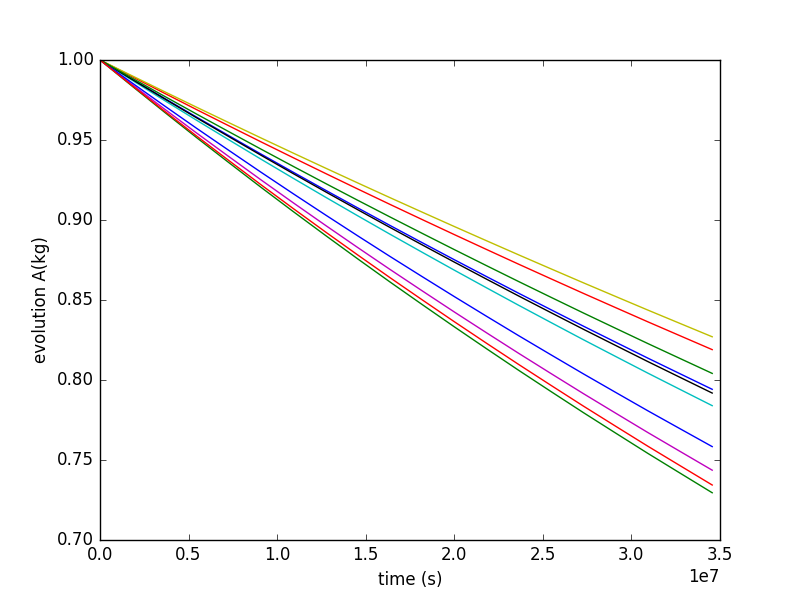
\includegraphics[scale=0.7]{../../tests/framework/user_guide/ravenTutorial/gold/ROMLoad/1-historyROMPlot_line.png}
  \caption{Plot of the histories generated by the Monte Carlo sampling of pickled ROM for variable $A$ (20 samples).}
  \label{fig:historiesROMPlotLine_A}
\end{figure}
%%%%%%%%%%%%%%%%%%%%%%%%%%%%%%%%%%%%%%%%%%%%%%%%%%%%%%%%%%

Finally, ROMs are generally not constructed for all possible inputs, geometries or representing all outputs. However,
it is possible to build a ROM of faster solution with respect to the original set. The accuracy in the prediction
can be obtained by further training. Figure~\ref{fig:romConstruction} shows the general workflow for ROM construction.

%%%%%%%%%%%%%%%%%%%%%%%%%%%%%%%%%%%%%%%%%%%%%%%%%%%%%%%%%%
%figure rom construction
\begin{figure}[h!]
  \centering
  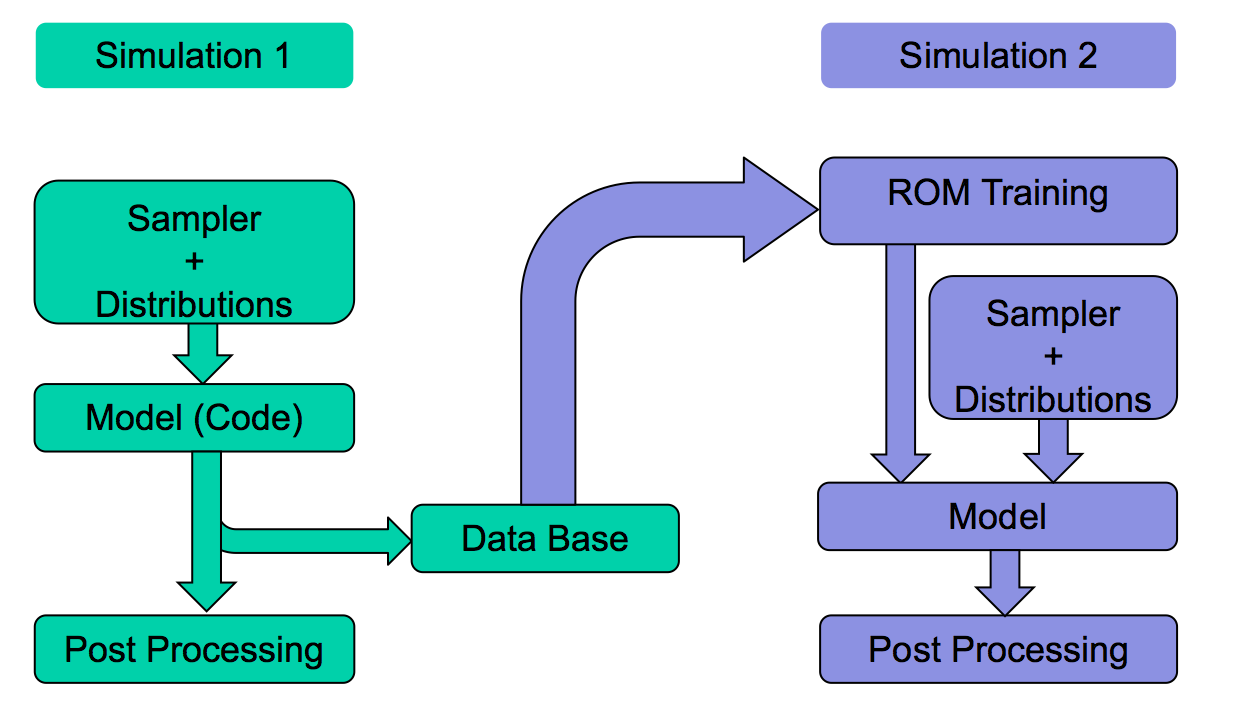
\includegraphics[scale=0.7]{./pics/romConstruction.png}
  \caption{Workflow for ROM construction}
  \label{fig:romConstruction}
\end{figure}
%%%%%%%%%%%%%%%%%%%%%%%%%%%%%%%%%%%%%%%%%%%%%%%%%%%%%%%%%%

\clearpage









